\documentclass{standalone}
\usepackage{fontspec}
\setsansfont{DejaVuSans.ttf}[Path=./,Kerning=Off,Ligatures={TeXOff,NoCommon}]
\usepackage{tikz}
\begin{document}
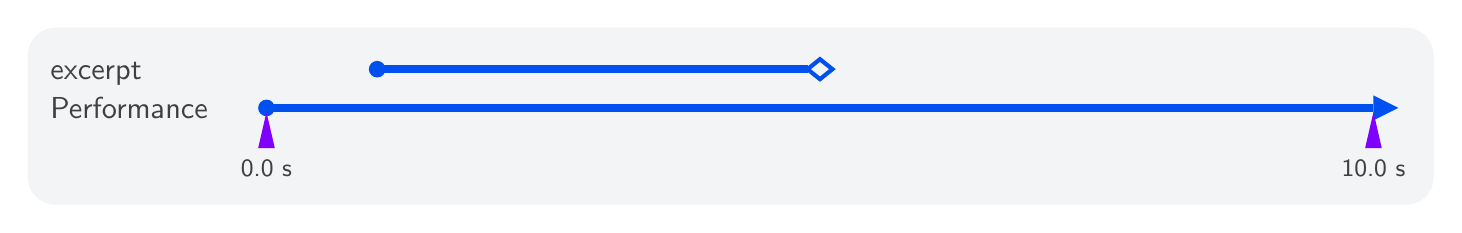
\begin{tikzpicture}[x=1pt,y=1pt,miter limit=4,font=\sffamily]
\definecolor{ts0050EF}{HTML}{0050EF}
\definecolor{ts404040}{HTML}{404040}
\definecolor{ts7F00FF}{HTML}{7F00FF}
\definecolor{tsF3F4F6}{HTML}{F3F4F6}
\begin{scope}[shift={(16,16)}]
\path[rounded corners=10pt,fill=tsF3F4F6] (0,0) rectangle (508.0859,63.9766);
\path[draw=ts0050EF,line width=3pt] (86.2915,34.9766) -- (486.2915,34.9766);
\path[fill=ts0050EF] (86.2915,34.9766) circle[radius=3];
\path[fill=ts0050EF] (495.2915,34.9766) -- (486.2915,39.4766) -- (486.2915,30.4766) -- cycle;
\path[draw=ts0050EF,line width=3pt] (126.2915,48.9766) -- (281.7915,48.9766);
\path[fill=ts0050EF] (126.2915,48.9766) circle[radius=3];
\path[draw=ts0050EF,line width=1.5pt] (281.7915,48.9766) -- (286.2915,52.5766) -- (290.7915,48.9766) -- (286.2915,45.3766) -- cycle;
\path[fill=ts7F00FF] (86.2915,33.4766) -- (83.2915,20.4766) -- (89.2915,20.4766) -- cycle;
\path[fill=ts7F00FF] (486.2915,33.4766) -- (483.2915,20.4766) -- (489.2915,20.4766) -- cycle;
\node[anchor=base west,inner sep=0,font=\sffamily\fontsize{11}{12.8047}\selectfont,text=ts404040] at (8,45.1685) {excerpt};
\node[anchor=base west,inner sep=0,font=\sffamily\fontsize{11}{12.8047}\selectfont,text=ts404040] at (8,31.1685) {Performance};
\node[anchor=base,inner sep=0,font=\sffamily\fontsize{9}{10.4766}\selectfont,text=ts404040] at (86.2915,10.1226) {0.0 s};
\node[anchor=base,inner sep=0,font=\sffamily\fontsize{9}{10.4766}\selectfont,text=ts404040] at (486.2915,10.1226) {10.0 s};
\end{scope}
\end{tikzpicture}
\end{document}
